\documentclass[]{article}
\usepackage{fullpage}
\usepackage{graphicx}
\usepackage{subcaption}
\usepackage{amsmath}
%opening
\title{Magnetohydrodynamic Cocktail Stirrer}
\author{Carlos Gross Jones}

\begin{document}

\maketitle

\begin{abstract}

\end{abstract}
\newpage
\section{Background}
\par The first attempt at a contactless cocktail was based on a simple application of the Lorentz force. Two copper electrodes placed in a glass tumbler passed a current through the liquid, while a strong magnet (a 2''x1''x3/4'' N45 block from United Nuclear Scientific LLC) under the tumbler provided an orthogonal magnetic field (Fig. \ref{fig:oldversion}). 
\begin{figure}
	\centering
	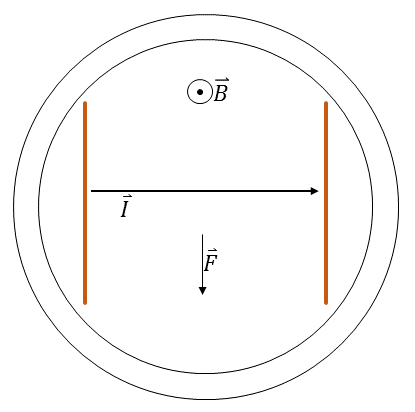
\includegraphics[width=0.5\textwidth]{Oldversion}
	\caption{First iteration of contactless stirrer}
	\label{fig:oldversion}
\end{figure}
Assuming time-invariance, the force applied on a differential element $\mathrm{d}V$ in a current field $\vec{J}$ and an orthogonal magnetic field $\vec{B}$ can be found from the element length d$\ell$ parallel to the current and cross-sectional area d$A$ normal to the current:
\begin{align}
\vec{F}=q\vec{V}\times\vec{B}\\
\vec{F}=I\vec{\ell}\times B\\
I=\lvert J\rvert\mathrm{d}A\\
\end{align}
(Valid because d$A$ is defined to be normal to $\vec{J}$.)
\begin{align}
\mathrm{d}\vec{F}=\lvert\vec{J}\rvert\mathrm{d}A\mathrm{d}\ell\times\vec{B}
\end{align}
Since, in this case, the magnetic and current fields are orthogonal, and since the current field is approximately uniform between the electrodes (simply the total current divided by the electrode area),
\begin{align}
\mathrm{d}\vec{F}=\lvert\vec{J}\rvert\lvert\vec{B}\rvert\mathrm{d}A\,\mathrm{d}\ell\\
\vec{F}=\iiint\limits_V\lvert\vec{J}\rvert\lvert\vec{B}\rvert\mathrm{d}A\,\mathrm{d}\ell
\end{align}
Given an electrode area of $A$ and spacing of $L$ and approximating both the current and magnetic field to be uniform between the electrodes,
\begin{align}
\vec{F}=\lvert\vec{B}\rvert L\iiint\limits_A\lvert\vec{J}\rvert\mathrm{d}A=\lvert\vec{B}\rvert IL
\end{align}
\par This design did work in principle; the Lorentz force produced a pumping action, where fluid would flow down the centerline between the electrodes and recirculate along the walls of the tumbler. However, since a large current was flowing through a fluid, significant electrolysis occurred, which, in addition to producing potentially dangerous hydrogen and oxygen gas, affected the taste of the cocktail due to the electrolysis products of ethanol.

\section{Theoretical Background}
\par Since the basic application of Lorentz force to pumping was effectively validated (and is in fact well studied \cite{yamato}), the major problem remaining was the electrolysis of the cocktail. As per Faraday's Law of Electrolysis:
\begin{equation}
\dot{m}=\frac{I}{F}\frac{M}{z}
\end{equation}
Where:
\begin{itemize}
	\item $\dot{m}$ is the mass of electrolysis products appearing at an electrode per unit time;
	\item $I$ is the total current flowing into or out of the electrode;
	\item $F$ is the Faraday constant, 96485 mol/C;
	\item $M$ is molar mass of the original substance;
	\item $z$ is the number of valence electrons of the substance.
\end{itemize}
\par Since $F$ is a constant and $M$ and $z$ are properties of the substance, in order to minimize $\dot{m}$, $I$ must be minimized. However, pumping force is also directly proportional to $I$. The central proposal of this project is that currents which circulate entirely within a fluid will not result in electrolysis, because the \textit{net} current flow through the fluid is zero. 
\par The obvious question is how to produce currents without an external EMF source such as a battery. The proposed solution is to use an external, time-variant magnetic field to induce circulating currents (eddy currents) in a conductive fluid.

\par For the purposes of a first-pass analysis, the following model will be considered:
\begin{itemize}
	\item The fluid will be a 3'' diameter, 3'' tall cylinder (based on an approximate cocktail tumbler);
	\item The fluid will be considered to have electrical resistivity $\rho$ and magnetic properties equal to a vacuum (water is in fact weakly diamagnetic, but this is expected to be a negligible contribution);
	\item A solenoid wound from copper wire surrounding the fluid will, when magnetized, produce a magnetic field $\vec{B_s}$ which is uniform throughout the fluid and parallel to the axis.
	\item As a practical consideration, the solenoid will be energized with standard 60 Hz power (the voltage, current, and limiting circuitry for the solenoid will be addressed later).
\end{itemize}

\par Since current in the coil is sinusoidal at 60 Hz, it will produce a solenoid magnetic field $B_s(t)$ (importantly, the field \emph{without} the effect of the central conductor) which oscillates at the same frequency (although not, of course, in phase):
\begin{equation}
B_s=B_{s,max}\cos(2\pi f t)=B_{max}\cos(120\pi t)
\end{equation}
and thus
\begin{equation}
\frac{\mathrm{d}B_s}{\mathrm{d}t}=-B_{s,max}120\pi\sin(120\pi t)
\label{eqn:dbdt}
\end{equation}
\par This time-variant magnetic field, when applied axially along a conductor, will induce eddy currents which orbit the axis. 

\subsection{Analysis of Induced Current Field}
\par The Maxwell-Faraday equation allows the tangential electric field around a closed contour $\partial\Sigma$ to be calculated from the magnetic field through the enclosed surface $\Sigma$:
\begin{equation}
\oint\limits_{\partial\Sigma}\vec{E}\cdot\mathrm{d}\ell = \left[ -\iint\limits_\Sigma\frac{\mathrm{d}\vec{B}}{\mathrm{d}t}\cdot\mathrm{d}\vec{A}\right] \,\hat{\theta}
\end{equation}
where the directions of $\partial\Sigma$ and $\vec{A}$ are related by the right-hand rule. Taking $\Sigma$ to be a slice of the liquid in the solenoid normal to the axis, $\vec{B}$ can be assumed to be uniform ($r$ independent) and normal to $\Sigma$, and $\vec{E}$ can be assumed to be perpendicular to $r$. 
\begin{align}
\vec{E}\oint\limits_{\partial\Sigma}\mathrm{d}\ell=-\left[ \frac{\mathrm{d}B}{\mathrm{d}t}\iint\limits_\Sigma\mathrm{d}\vec{A}\right]\,\hat{\theta}\\
\vec{E} 2\pi r=-\frac{\mathrm{d}B}{\mathrm{d}t}\pi r^2\,\hat{\theta}\\
\vec{E}=-\frac{\mathrm{d}B}{\mathrm{d}t}\frac{r}{2}\,\hat{\theta}\\
\end{align}
Applying the known resistivity,
\begin{align}
\vec{J} = \frac{\vec{E}}{\rho}\\
\vec{J}=-\frac{\mathrm{d}B}{\mathrm{d}t}\frac{r}{2\rho}\,\hat{\theta}
\end{align}
Combining with \ref{eqn:dbdt},
\begin{align}
\vec{J}=B_{s,max}\sin(120\pi t)\frac{120\pi r}{2\rho}\,\hat{\theta}
\label{eqn:simpleJ}\\
\vec{J}_{max}=B_{s,max}\frac{120\pi r}{2\rho}\,\hat{\theta}
\label{eqn:simpleJmax}
\end{align}
\par Therefore, for the circuit $\partial\Sigma$ inside the solenoid, current is expected to be directly proportional to $B_{s,max}$ and $r$, and inversely proportional to $\rho$. However, this relation cannot necessarily be used to compute the current field. While it is valid for a single conducting ring, it does not take into account the \emph{demagnetizing} (opposite $B_{s}$) field created by other induced currents inside $\Sigma$. While it is possible to analytically compute the current field (via magnetic vector potential) in a finite conducting rod \cite{analyticeddy}, in this case it is possible to neglect the secondary magnetic fields created by eddy currents. In other words, due to the effects of currents in the conductor, the net magnetic field within the cylinder ceases to be uniform.
\par To validate this assumption, finite-element analysis will be used to characterize the current field within the medium. Assuming the system is rotationally symmetric, the currents can be described by current intensity normal to a radial plane, and therefore 2D FEA in an axisymmetric coordinate system is sufficient. In this case, FEMM (Finite Element Method Magnetics) was chosen to model the system, with a time-harmonic frequency of 60 Hz and the coil modeled as a hollow cylinder of copper with homogeneous current density. 
\par As an example of the net magnetic field distribution and induced current field in a good conductor (the situation analyzed in \cite{analyticeddy}), the ``liquid'' in the tumbler is first modeled as a copper block.
\begin{figure}[h]
	\centering
	\begin{subfigure}{0.45\textwidth}
		\centering
		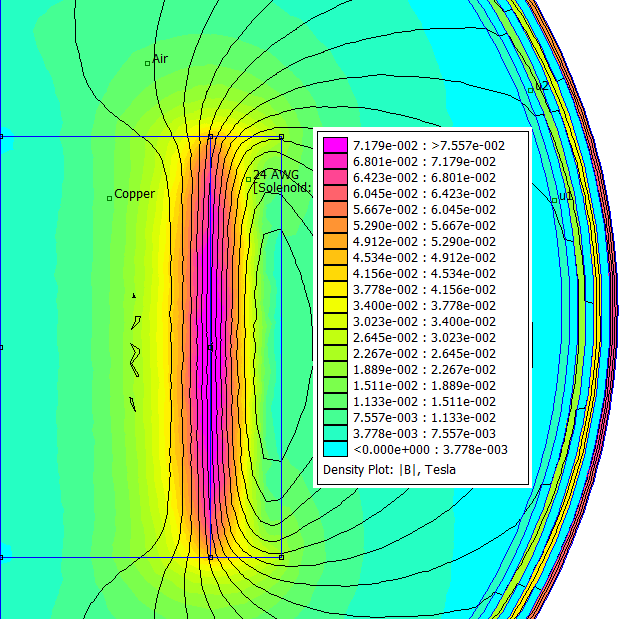
\includegraphics[width=1\textwidth]{CopperB}
		\caption{Magnetic field density}
		\label{fig:copperb}
	\end{subfigure}
	\begin{subfigure}{0.45\textwidth}
		\centering
		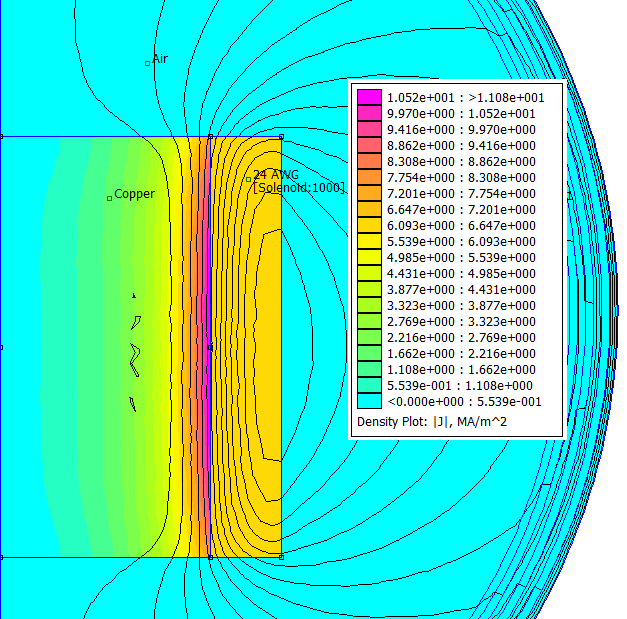
\includegraphics[width=1\textwidth]{CopperJ}
		\caption{Induced current density}
		\label{fig:copperj}
	\end{subfigure}
	\caption{Copper cylinder in solenoid field at 60 Hz}
\end{figure}
As shown in Fig. \ref{fig:copperb}, the net magnetic field within the copper block is very different from the uniform field generated by the solenoid. (Since both the magnetic and induced current fields are sinusoidal, all graphical plots, unless otherwise stated, show the peak magnitude; phase is not shown.) As expected with increasing conductance, the block begins to ``exclude'' the magnetic field (with superconductors, of course, excluding external magnetic fields entirely). As a result, the current density along a radius of the block (at $z=h/2$) (Fig. \ref{fig:copperjgraph}) is definitely not of the $1/r$ form predicted by Eqn. \ref{eqn:simpleJ}.
\begin{figure}[h]
	\centering
	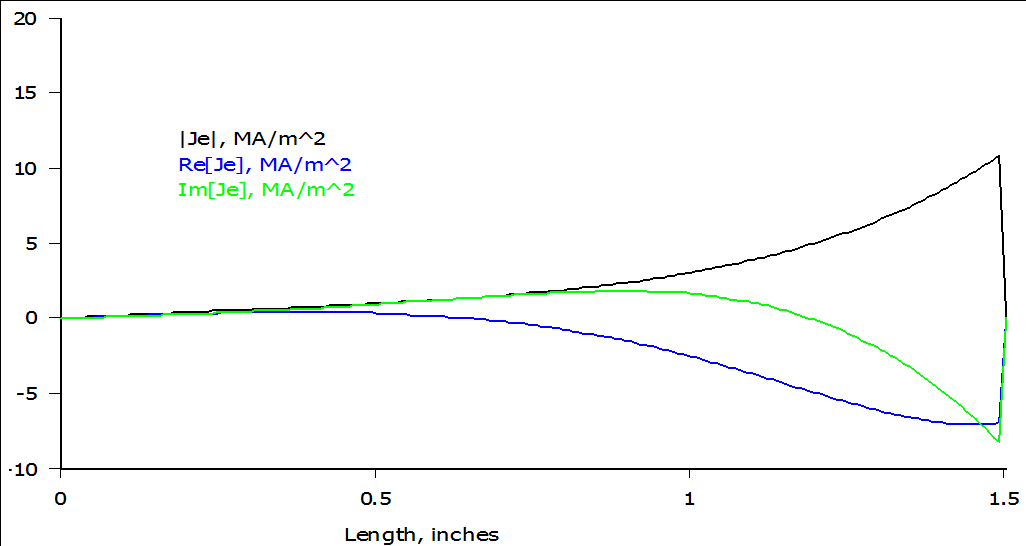
\includegraphics[width=0.7\textwidth]{CopperJgraph}
	\caption{Plot of current density versus radius in copper cylinder}
\end{figure}
\par This situation would be best modeled using modified Bessel functions as described in \cite{analyticeddy}. However, when the copper ($\rho =1.68\cdot 10^{-8}\, \Omega\cdot\textrm{m}$) is replaced by much less conductive seawater ($\rho =0.2\, \Omega\cdot\textrm{m}$), the influence of secondary magnetic fields on $B_{s}$ becomes negligible (Fig. \ref{fig:seawaterb}).
\begin{figure}[h]
	\centering
	\begin{subfigure}{0.45\textwidth}
		\centering
		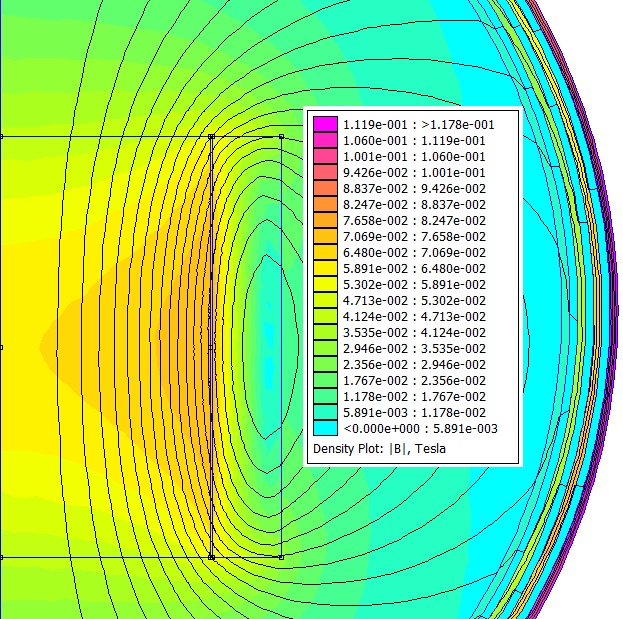
\includegraphics[width=1\textwidth]{SeawaterB}
		\caption{Magnetic field density}
		\label{fig:seawaterb}
	\end{subfigure}
	\begin{subfigure}{0.45\textwidth}
		\centering
		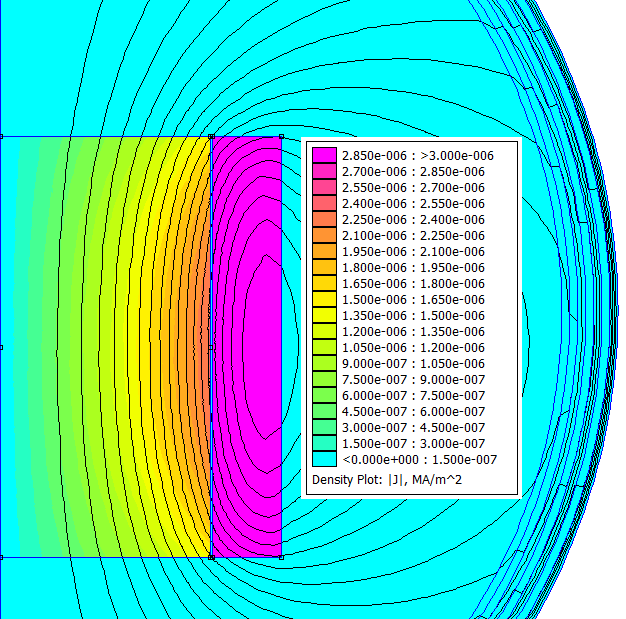
\includegraphics[width=1\textwidth]{SeawaterJ}
		\caption{Induced current density}
		\label{fig:seawaterj}
	\end{subfigure}
	\caption{Seawater in solenoid field at 60 Hz}
\end{figure}
Therefore, the peak current density matches Eqn. \ref{eqn:simpleJmax} fairly well (Fig. \ref{fig:seawaterJcomparison}).
\begin{figure}
	\centering
	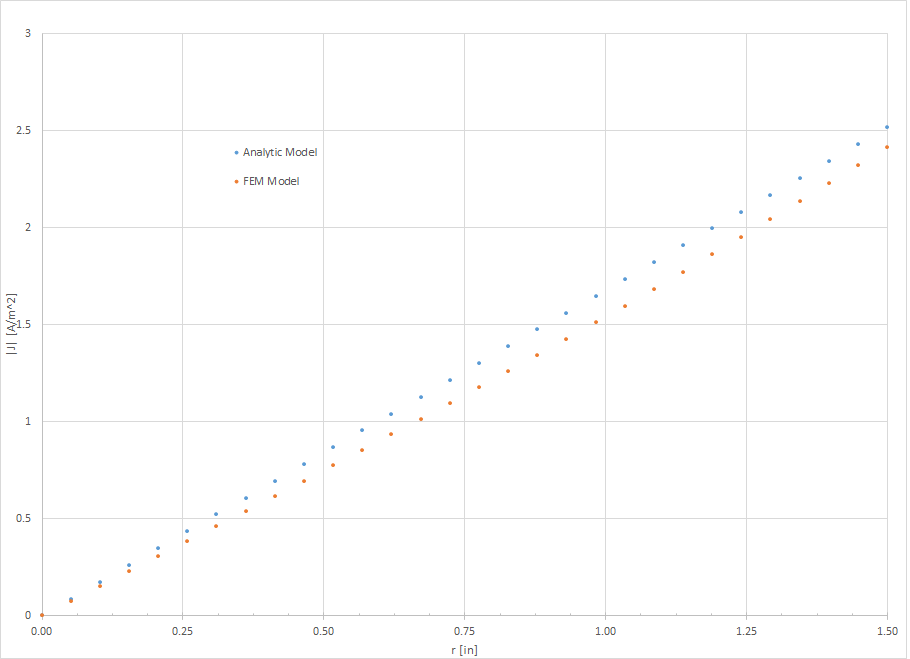
\includegraphics[width=1\textwidth]{SeawaterJComparison}
	\caption{Plot of $J_{max}$ in seawater as predicted by analytic model (Eqn. \ref{eqn:simpleJmax}) and FEM model}
	\label{fig:seawaterJcomparison}
\end{figure}

\par Since, at this point, the goal is to find the form of the current field and its dependence on $B_{s,max}$ and $\rho$, it is not necessary to accurately know the resistivity of an actual cocktail; those values are calculated later in \S\ref{sec:resistivity}.

\subsection{General Design}
\par While effectively solving the electrolysis problem, this prohibits the simple structure of the original design: since the currents in the liquid now oscillate sinusoidally at 60 Hz, in a static $\vec{B}$ field, the force on a parcel of liquid would also oscillate, producing no net motion. Therefore, the applied magnetic field must oscillate as well, synchronous with the solenoid current. The simplest design of this type would have a second electromagnet mounted orthogonally to the first, and driven from the same power source. However, geometry would require either a single large solenoid outside the axial solenoid, or two smaller solenoids (presumably with ferrous cores) on either side of the tumbler. The first case would require impractical amount of wire to construct, and the second generates a frustratingly weak field through the liquid. Therefore, large permanent magnets were next considered. 3'' dia. x 1'' thick NdFeB45 magnets from United Nuclear Scientific LLC were chosen based on field strength per dollar (\$140 and maximum $\vec{B}\cdot\vec{n}$ of $\approx$0.42 T).

\section{Solenoid Design}
\section{Rotor Design}

\section{Property Measurements}
\subsection{Cocktail Resistivity}
\label{sec:resistivity}
\subsection{$\vec{B_s}$ Measurement}
\subsection{Rotor Field Measurement}



\begin{thebibliography}{3}
	\bibitem{yamato}
	Takezawa, Setsuo et al. ``Operation of the Thruster for Superconducting Electromagnetohydrodynamic Propulsion Ship YAMATO 1.'' Bulletin of the M.E.S.J 23.1 (1993): 46-55. Japan Institute of Marine Engineering. Web. 21 Aug. 2016. \textless http://www.jime.jp/e/publication/bulletin/english/pdf/mv23n011995p46.pdf>.\textgreater
	
	\bibitem{curesistivity}
	Matula, R. A. ``Electrical Resistivity of Copper, Gold, Palladium, and Silver.'' \textit{Journal of Physical and Chemical Reference Data} 8.4 (1979): 1161. Web. 23 Aug. 2016. \textless http://www.nist.gov/data/PDFfiles/jpcrd155.pdf\textgreater. 
	
	\bibitem{analyticeddy}
	Bowler, John R., and Theodoros P. Theodoulidis. ``Eddy Currents Induced in a Conducting Rod of Finite Length by a Coaxial Encircling Coil.'' Journal of Physics D: Applied Physics 38.16 (2005): 2861-868. Web. 23 Aug. 2016. 
\end{thebibliography}
\end{document}
